\documentclass[11pt]{article}
\usepackage[utf8]{inputenc}
\usepackage[T1]{fontenc}
\usepackage[margin=2.4cm]{geometry}
\usepackage{booktabs}
\usepackage{amsmath}
\usepackage{graphicx}
\usepackage{float}
\graphicspath{{figures/}}
\setlength{\parskip}{0.5em}
\setlength{\parindent}{0pt}

\title{\vspace{-2.5em}Efecto de la transformaci\'on de Box--Cox en la segmentaci\'on de grietas}
\author{}
\date{}

\begin{document}
\maketitle
\vspace{-3em}

Este informe resume el efecto de la transformaci\'on de Box--Cox como prefiltrado en la
segmentaci\'on de grietas, evaluado sobre cuatro conjuntos de im\'agenes seg\'un la geometr\'ia
de la fractura. Se reportan los datos, la metodolog\'ia y los resultados, con \'enfasis en
c\'omo la transformaci\'on \textbf{mejora la capacidad de detecci\'on de la grieta
(\emph{recall})} y en el compromiso resultante con la \emph{precision}.

\section*{1. Datos}
Utilic\'e el conjunto de grietas de hormig\'on de \"Ozgenel \& Sorgu\c{c}. Seleccion\'e
\textbf{cuatro conjuntos de 50 im\'agenes} seg\'un la geometr\'ia de la fractura:
\textbf{verticales}, \textbf{horizontales}, \textbf{oblicuas} (de izquierda a derecha) y
\textbf{grandes} (la grieta ocupa una porci\'on amplia de la imagen). Cada imagen RGB tiene su
m\'ascara binaria (grieta \emph{vs.} fondo). Todas se redimensionaron a $256\times256$ y la
m\'ascara se binariz\'o. En total, $4\times50=200$ im\'agenes etiquetadas.

\section*{2. Metodolog\'ia}
\textbf{Prefiltrado Box--Cox.} Cada imagen se convierte a escala de grises
($0{,}299R+0{,}587G+0{,}114B$), se le aplica la transformaci\'on de Box--Cox con $\lambda$
estimado por m\'axima verosimilitud y luego un \emph{histogram stretching} a $[0,1]$. La
transformaci\'on es \textbf{por imagen} (cada una con su propio $\lambda$). Comparo dos
condiciones: \textbf{sin} Box--Cox (intensidad gris cruda) y \textbf{con} Box--Cox.

\textbf{Clasificadores.} Cinco m\'etodos cl\'asicos a nivel de p\'ixel: SVM (RBF), LightGBM,
KNN, LDA y QDA. La \emph{feature} es la intensidad del p\'ixel. \textbf{Protocolo por imagen}:
para cada imagen se entrena con una muestra estratificada de sus p\'ixeles y se predice la
imagen completa, siguiendo el protocolo del art\'iculo original.

\textbf{M\'etricas} (clase grieta): IoU, Dice/F1, \emph{Precision} y \emph{Recall}. Reporto
\textbf{media\,$\pm$\,desviaci\'on est\'andar sobre las 50 im\'agenes} de cada conjunto.
La \emph{Accuracy} se omite por ser enga\~nosa (la grieta es $\sim$1\,\% de los p\'ixeles).

\textbf{Significancia.} Para cada comparaci\'on con/sin Box--Cox uso un \textbf{test pareado de
permutaci\'on} (sign-flip) y el de Wilcoxon, ambos pareando imagen con imagen, m\'as
\textbf{intervalos de confianza al 95\,\% por bootstrap}. El bootstrap es v\'alido aqu\'i porque
se remuestrean \emph{im\'agenes} (observaciones independientes), no p\'ixeles de una misma
imagen (que presentan autocorrelaci\'on espacial). Significancia: $^{*}p<0{,}05$,
$^{**}p<0{,}01$, $^{***}p<0{,}001$.

\section*{3. Resultados}
\begin{table}[H]\centering\small
\caption{Calidad global de la segmentaci\'on de la grieta: IoU y Dice (F1), media\,$\pm$\,desv.\ est.\ sobre las 50 im\'agenes de cada conjunto. $\Delta=$ con\,$-$\,sin Box--Cox (puntos porcentuales).}\label{tab:iou}
\begin{tabular}{l ccc ccc}
\toprule
M\'etodo & \multicolumn{3}{c}{IoU (\%)} & \multicolumn{3}{c}{Dice (\%)} \\
\cmidrule(lr){2-4}\cmidrule(lr){5-7}
 & sin BC & con BC & $\Delta$ & sin BC & con BC & $\Delta$ \\
\midrule
\multicolumn{7}{l}{\textit{Verticales} ($\bar\lambda=2.17$)} \\
\quad SVM & $37.8\pm13.0$ & $36.7\pm12.7$ & $-1.1$$^{***}$ & $53.6\pm14.2$ & $52.4\pm14.1$ & $-1.2$$^{***}$ \\
\quad LightGBM & $29.4\pm11.5$ & $29.3\pm11.4$ & $-0.1$ & $44.3\pm13.4$ & $44.2\pm13.3$ & $-0.1$ \\
\quad KNN & $24.7\pm11.0$ & $24.7\pm11.0$ & $+0.0$ & $38.4\pm13.4$ & $38.5\pm13.4$ & $+0.1$ \\
\quad LDA & $41.3\pm16.1$ & $32.9\pm13.6$ & $-8.4$$^{***}$ & $56.6\pm17.2$ & $48.0\pm16.1$ & $-8.7$$^{***}$ \\
\quad QDA & $39.0\pm17.4$ & $37.6\pm16.5$ & $-1.4$ & $53.7\pm19.6$ & $52.4\pm19.0$ & $-1.3$ \\
\addlinespace
\multicolumn{7}{l}{\textit{Horizontales} ($\bar\lambda=1.73$)} \\
\quad SVM & $32.6\pm10.2$ & $32.2\pm9.9$ & $-0.4$$^{***}$ & $48.3\pm11.6$ & $47.9\pm11.3$ & $-0.4$$^{***}$ \\
\quad LightGBM & $26.8\pm9.6$ & $26.7\pm9.2$ & $-0.1$ & $41.4\pm11.8$ & $41.3\pm11.4$ & $-0.1$ \\
\quad KNN & $21.5\pm7.3$ & $21.5\pm7.3$ & $+0.0$ & $34.8\pm9.7$ & $34.8\pm9.7$ & $+0.0$ \\
\quad LDA & $34.9\pm12.9$ & $29.8\pm10.2$ & $-5.1$$^{***}$ & $50.4\pm14.4$ & $45.0\pm11.9$ & $-5.4$$^{***}$ \\
\quad QDA & $32.2\pm15.9$ & $34.6\pm13.3$ & $+2.4$$^{*}$ & $46.4\pm20.2$ & $49.9\pm16.2$ & $+3.5$$^{**}$ \\
\addlinespace
\multicolumn{7}{l}{\textit{Oblicuas (izq.\,$\to$\,der.)} ($\bar\lambda=2.11$)} \\
\quad SVM & $37.4\pm12.2$ & $36.4\pm11.6$ & $-1.1$$^{***}$ & $53.3\pm13.4$ & $52.3\pm13.0$ & $-1.1$$^{***}$ \\
\quad LightGBM & $30.4\pm10.7$ & $30.5\pm10.7$ & $+0.1$ & $45.5\pm13.0$ & $45.7\pm12.9$ & $+0.1$ \\
\quad KNN & $23.9\pm8.7$ & $23.9\pm8.7$ & $-0.0$ & $37.8\pm11.5$ & $37.8\pm11.5$ & $-0.0$ \\
\quad LDA & $40.7\pm17.1$ & $29.5\pm12.0$ & $-11.2$$^{***}$ & $55.7\pm18.5$ & $44.2\pm14.4$ & $-11.4$$^{***}$ \\
\quad QDA & $41.0\pm16.3$ & $39.0\pm13.2$ & $-2.1$ & $56.1\pm18.2$ & $54.8\pm14.3$ & $-1.4$ \\
\addlinespace
\multicolumn{7}{l}{\textit{Grandes} ($\bar\lambda=2.38$)} \\
\quad SVM & $32.5\pm10.5$ & $31.5\pm9.9$ & $-1.0$$^{***}$ & $48.1\pm12.4$ & $47.0\pm11.9$ & $-1.1$$^{***}$ \\
\quad LightGBM & $25.8\pm7.7$ & $25.8\pm7.8$ & $-0.1$ & $40.5\pm9.7$ & $40.4\pm9.7$ & $-0.1$ \\
\quad KNN & $20.5\pm6.1$ & $20.4\pm6.1$ & $-0.1$$^{**}$ & $33.6\pm8.1$ & $33.5\pm8.1$ & $-0.1$$^{**}$ \\
\quad LDA & $36.2\pm11.9$ & $25.0\pm8.9$ & $-11.3$$^{***}$ & $52.1\pm13.2$ & $39.2\pm11.2$ & $-12.9$$^{***}$ \\
\quad QDA & $37.6\pm10.8$ & $33.1\pm11.2$ & $-4.4$$^{***}$ & $53.7\pm11.6$ & $48.7\pm12.8$ & $-5.0$$^{***}$ \\
\bottomrule
\end{tabular}
\end{table}

\begin{table}[H]\centering\small
\caption{Compromiso \emph{precision}--\emph{recall} para la clase grieta, media\,$\pm$\,desv.\ est.\ sobre 50 im\'agenes. $\Delta=$ con\,$-$\,sin Box--Cox.}\label{tab:pr}
\begin{tabular}{l ccc ccc}
\toprule
M\'etodo & \multicolumn{3}{c}{Precision (\%)} & \multicolumn{3}{c}{Recall (\%)} \\
\cmidrule(lr){2-4}\cmidrule(lr){5-7}
 & sin BC & con BC & $\Delta$ & sin BC & con BC & $\Delta$ \\
\midrule
\multicolumn{7}{l}{\textit{Verticales} ($\bar\lambda=2.17$)} \\
\quad SVM & $47.8\pm14.6$ & $45.8\pm14.2$ & $-1.9$$^{***}$ & $63.2\pm15.0$ & $63.6\pm15.2$ & $+0.5$$^{***}$ \\
\quad LightGBM & $33.9\pm12.5$ & $33.8\pm12.4$ & $-0.1$ & $67.4\pm14.7$ & $67.4\pm14.6$ & $+0.0$ \\
\quad KNN & $27.0\pm11.6$ & $27.1\pm11.6$ & $+0.1$ & $70.8\pm12.9$ & $70.8\pm13.0$ & $+0.0$ \\
\quad LDA & $58.2\pm21.1$ & $42.6\pm19.7$ & $-15.6$$^{***}$ & $59.0\pm12.9$ & $64.5\pm16.1$ & $+5.5$$^{***}$ \\
\quad QDA & $74.6\pm21.8$ & $61.3\pm23.4$ & $-13.3$$^{***}$ & $45.6\pm19.1$ & $53.7\pm21.5$ & $+8.1$$^{***}$ \\
\addlinespace
\multicolumn{7}{l}{\textit{Horizontales} ($\bar\lambda=1.73$)} \\
\quad SVM & $43.0\pm12.0$ & $42.3\pm11.8$ & $-0.7$$^{***}$ & $57.1\pm13.5$ & $57.3\pm13.6$ & $+0.2$$^{***}$ \\
\quad LightGBM & $32.3\pm11.1$ & $32.2\pm10.7$ & $-0.1$ & $60.4\pm13.0$ & $60.4\pm13.1$ & $-0.0$ \\
\quad KNN & $24.3\pm7.9$ & $24.3\pm7.9$ & $+0.0$ & $63.8\pm12.2$ & $63.8\pm12.3$ & $+0.0$ \\
\quad LDA & $48.5\pm17.4$ & $39.3\pm14.1$ & $-9.2$$^{***}$ & $54.7\pm11.7$ & $57.6\pm14.6$ & $+2.9$$^{***}$ \\
\quad QDA & $77.8\pm10.6$ & $63.5\pm17.3$ & $-14.3$$^{***}$ & $37.0\pm19.6$ & $46.4\pm19.8$ & $+9.4$$^{***}$ \\
\addlinespace
\multicolumn{7}{l}{\textit{Oblicuas (izq.\,$\to$\,der.)} ($\bar\lambda=2.11$)} \\
\quad SVM & $48.4\pm14.8$ & $46.4\pm13.9$ & $-2.0$$^{***}$ & $61.7\pm13.9$ & $62.2\pm14.1$ & $+0.5$$^{***}$ \\
\quad LightGBM & $36.1\pm12.7$ & $36.3\pm12.6$ & $+0.2$ & $65.2\pm13.4$ & $65.0\pm13.6$ & $-0.2$ \\
\quad KNN & $26.5\pm9.5$ & $26.5\pm9.5$ & $-0.0$ & $69.5\pm11.0$ & $69.5\pm11.0$ & $-0.0$ \\
\quad LDA & $56.6\pm24.4$ & $36.5\pm17.0$ & $-20.1$$^{***}$ & $59.1\pm11.1$ & $64.2\pm14.2$ & $+5.1$$^{***}$ \\
\quad QDA & $78.8\pm19.9$ & $61.3\pm19.8$ & $-17.4$$^{***}$ & $45.9\pm17.2$ & $55.5\pm17.6$ & $+9.6$$^{***}$ \\
\addlinespace
\multicolumn{7}{l}{\textit{Grandes} ($\bar\lambda=2.38$)} \\
\quad SVM & $42.2\pm15.5$ & $40.2\pm14.5$ & $-2.0$$^{***}$ & $63.7\pm12.1$ & $64.2\pm12.1$ & $+0.6$$^{***}$ \\
\quad LightGBM & $30.3\pm9.8$ & $30.2\pm9.8$ & $-0.1$ & $66.9\pm10.7$ & $67.0\pm10.7$ & $+0.0$ \\
\quad KNN & $22.4\pm6.9$ & $22.3\pm6.9$ & $-0.1$$^{**}$ & $71.0\pm7.2$ & $71.0\pm7.1$ & $+0.0$$^{*}$ \\
\quad LDA & $52.4\pm18.9$ & $30.6\pm14.3$ & $-21.8$$^{***}$ & $56.3\pm8.3$ & $65.2\pm11.0$ & $+8.9$$^{***}$ \\
\quad QDA & $67.9\pm17.0$ & $48.1\pm19.1$ & $-19.9$$^{***}$ & $46.4\pm10.7$ & $58.2\pm13.5$ & $+11.8$$^{***}$ \\
\bottomrule
\end{tabular}
\end{table}

\section*{4. Efecto de la transformaci\'on: mejora del \emph{recall}}
El efecto de Box--Cox es \textbf{sistem\'atico y coherente en los cuatro conjuntos}: al estirar
el contraste de los p\'ixeles oscuros de la grieta, la transformaci\'on \textbf{realza la
fractura respecto del fondo} y el clasificador \textbf{reconoce m\'as p\'ixeles que realmente
son grieta}. En consecuencia, el \textbf{\emph{recall} aumenta de forma significativa} en todos
los conjuntos (menos falsos negativos): mejora la capacidad de \emph{detectar} la fractura. El
costo es una ca\'ida de la \emph{precision} (m\'as fondo etiquetado como grieta), por lo que el
resultado neto es el cl\'asico \textbf{compromiso \emph{precision}--\emph{recall}}: se gana
sensibilidad de detecci\'on a cambio de una localizaci\'on m\'as gruesa de la grieta.

El tama\~no del efecto depende del m\'etodo:
\begin{itemize}
  \item \textbf{LDA y QDA} (sensibles a la distribuci\'on, pues asumen normalidad) muestran el
  efecto m\'as marcado: el \emph{recall} sube entre $+5$ y $+12$ puntos, pero la
  \emph{precision} cae a\'un m\'as (entre $-9$ y $-22$ puntos). Como la p\'erdida de
  \emph{precision} domina, el \textbf{IoU y el Dice empeoran}.
  \item \textbf{SVM} muestra un cambio peque\~no en la misma direcci\'on ($\sim+0{,}5$ de
  \emph{recall}, $\sim-2$ de \emph{precision}); IoU/Dice bajan levemente.
  \item \textbf{LightGBM y KNN} son pr\'acticamente \textbf{invariantes} ($\Delta\approx0$), como
  cabe esperar de m\'etodos insensibles a transformaciones mon\'otonas de una sola
  \emph{feature}.
\end{itemize}

\section*{5. Ejemplos}
Un ejemplo por tipo de grieta (clasificador QDA). De izquierda a derecha: imagen RGB, m\'ascara
real y segmentaci\'on \emph{sin} y \emph{con} Box--Cox. Con la transformaci\'on el modelo
reconoce m\'as p\'ixeles de grieta (mayor \emph{recall}); en el caso oblicuo, sin Box--Cox no se
detecta nada y la transformaci\'on lo \emph{rescata}.

\begin{figure}[H]\centering
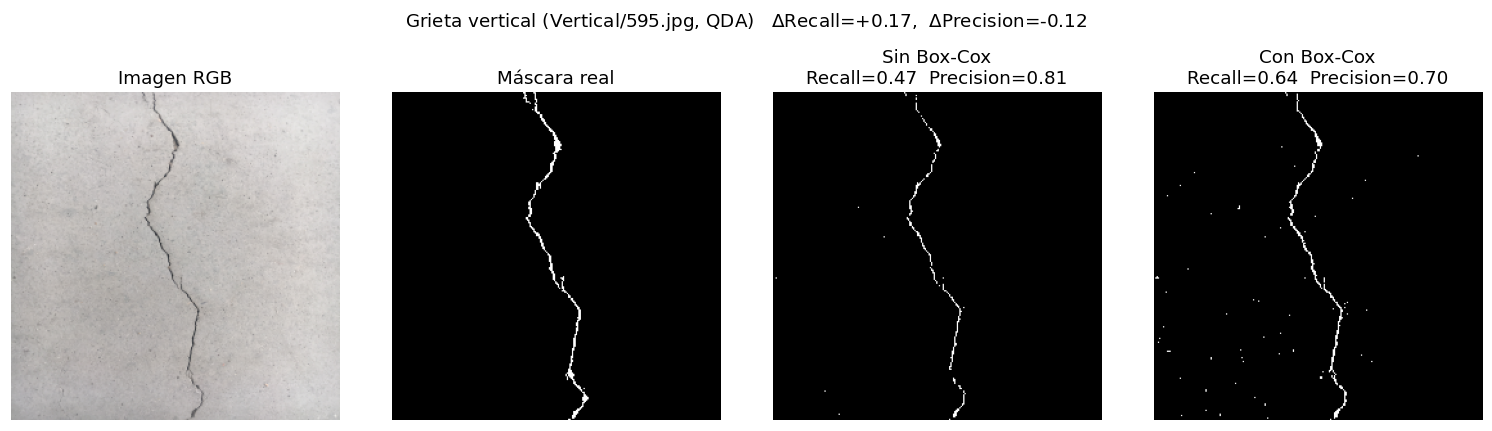
\includegraphics[width=\linewidth]{ej_Vertical.png}
\caption{Grieta vertical.}
\end{figure}

\begin{figure}[H]\centering
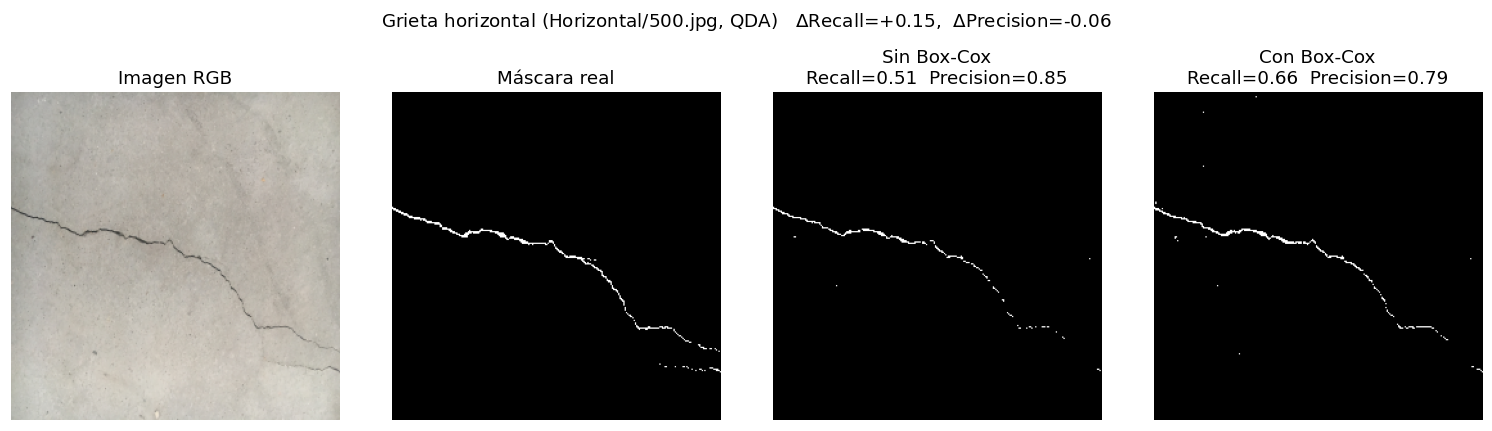
\includegraphics[width=\linewidth]{ej_Horizontal.png}
\caption{Grieta horizontal.}
\end{figure}

\begin{figure}[H]\centering
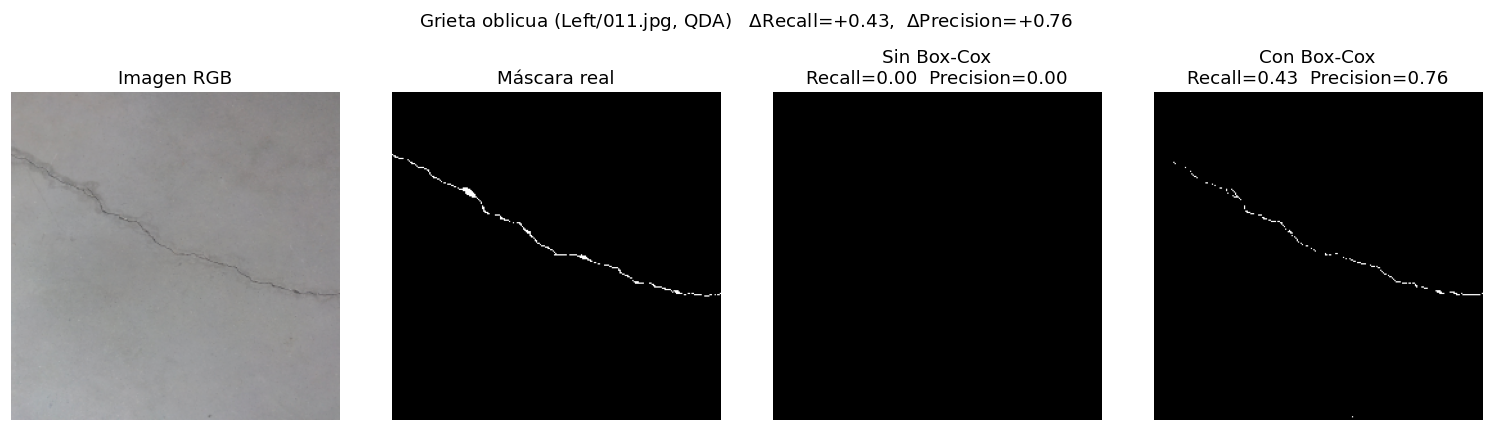
\includegraphics[width=\linewidth]{ej_Left.png}
\caption{Grieta oblicua (caso de rescate: sin Box--Cox no se detecta nada).}
\end{figure}

\begin{figure}[H]\centering
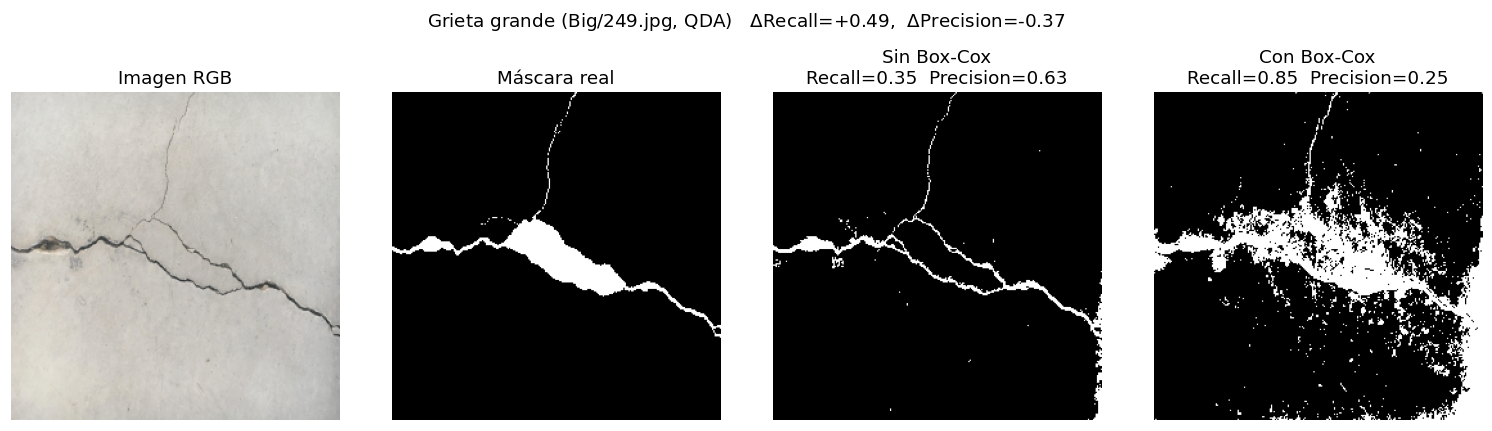
\includegraphics[width=\linewidth]{ej_Big.png}
\caption{Grieta grande.}
\end{figure}

\section*{6. Resultados por tipo de grieta}
\begin{itemize}
  \item \textbf{Verticales:} Box--Cox aumenta el \emph{recall} de QDA ($+8{,}1$) y LDA ($+5{,}5$),
  pero la ca\'ida de \emph{precision} ($-13{,}3$ y $-15{,}6$) reduce el IoU (LDA $-8{,}4$;
  QDA $-1{,}4$, no significativo). El resto sin cambios relevantes.
  \item \textbf{Horizontales:} \emph{\'Unico caso favorable.} En QDA, el fuerte aumento de
  \emph{recall} ($+9{,}4$) compensa la p\'erdida de \emph{precision} y el \textbf{IoU sube
  $+2{,}4$ y el Dice $+3{,}5$} (significativos, $p<0{,}05$). LDA sigue empeorando ($-5{,}1$).
  \item \textbf{Oblicuas:} comportamiento similar a verticales; LDA es el m\'as perjudicado
  (IoU $-11{,}2$, \emph{precision} $-20{,}1$) pese a ganar \emph{recall} ($+5{,}1$).
  \item \textbf{Grandes:} el \textbf{caso m\'as desfavorable}. LDA (IoU $-11{,}3$) y QDA
  (IoU $-4{,}4$) caen claramente: aunque el \emph{recall} sube mucho (QDA $+11{,}8$), la
  \emph{precision} se desploma ($-21{,}8$ y $-19{,}9$).
\end{itemize}

\section*{7. Conclusi\'on}
Sobre un conjunto de prueba amplio (50 im\'agenes por tipo, con medidas de incertidumbre y tests
pareados), Box--Cox \textbf{mejora la detecci\'on de la grieta}: aumenta el \emph{recall} de
forma significativa en los cuatro tipos, especialmente en los clasificadores sensibles a la
distribuci\'on (LDA y QDA), e incluso \textbf{rescata} casos en que sin la transformaci\'on el
modelo no detecta nada. El contrapeso es una p\'erdida de \emph{precision}: la regi\'on predicha
se engrosa e incorpora fondo, por lo que en agregado el IoU y el Dice pueden bajar (salvo QDA en
grietas horizontales, donde el balance es favorable). La transformaci\'on es, por tanto,
especialmente \'util cuando la prioridad es \textbf{no pasar por alto la fractura} (maximizar
\emph{recall}); si se requiere una delimitaci\'on m\'as fina, conviene combinarla con un
post-procesamiento que recupere \emph{precision}. Los m\'etodos basados en \'arboles o vecinos
(LightGBM, KNN) son insensibles a la transformaci\'on.

\end{document}
